\documentclass[letter]{article}
\usepackage{amsmath}
\usepackage{amsfonts}
\usepackage{amssymb}
\usepackage{ifthen}
\usepackage{fancyhdr}
\usepackage[usenames,dvipsnames,svgnames,table]{xcolor}
\usepackage{tikz}

%%%
% Set up the margins to use a fairly large area of the page
%%%
\oddsidemargin=.2in
\evensidemargin=.2in
\textwidth=6in
\topmargin=0in
\textheight=9.0in
\parskip=.07in
\parindent=0in
\pagestyle{fancy}

\expandafter\def\expandafter\quote\expandafter{\quote\sf\color{DarkGreen}}

%%%
% Set up the header
%%%
\newcommand{\setheader}[6]{
  \lhead{{\sc #1}\\{\sc #2} %({\small \it \today})
  }
  \rhead{
    {\bf #3}
    \ifthenelse{\equal{#4}{}}{}{(#4)}\\
    {\bf #5}
    \ifthenelse{\equal{#6}{}}{}{(#6)}%
  }
}

%%%
% Set up some shortcut commands
%%%
\newcommand{\R}{\mathbb{R}}
\newcommand{\N}{\mathbb{N}}
\newcommand{\Z}{\mathbb{Z}}
\newcommand{\Proj}{\mathrm{proj}}
\newcommand{\Perp}{\mathrm{perp}}
\newcommand{\Span}{\mathrm{span}}
\newcommand{\Null}{\mathrm{null}}
\newcommand{\Rank}{\mathrm{rank}}
\newcommand{\mat}[1]{\begin{bmatrix}#1\end{bmatrix}}

%%%
% This is where the body of the document goes
%%%
\begin{document}
  \setheader{Math 211 (A01)}{Typed Homework 2}{Due Friday, February 20}{}{Bill Xiong, Arlene Zhang}{V00737042,V00802761}


\section{Question 1}
We know a system of linear equations can have $0,1$, or infinitely many solutions.
      \begin{enumerate}
        \item Explain why a system of linear equations cannot have exactly 2 solutions.
        \item For a homogeneous system of linear equations, what are the possibilities
          for the number of solutions?  Explain, and make sure to define
          \emph{homogeneous system}.
      \end{enumerate}

\subsection{Solution for Q1.1}
By definition, the individual equations that make up the system of equations in question have to be linear. This is, after all, \emph{linear} algebra.

Also by definition, lines can intercept other lines either at exactly one point, at infinite points (ie, two lines right on top of one another), or not at all (two lines parallel to each other). For a system to have exactly two solutions would require two points of interception, which would mean that one of the two equations plots to a parabola when graphed, making it nonlinear.

Thus, a system of linear equations cannot have exactly two solutions.

\subsection{Solution for Q1.2}
Recall that a system of linear equations is called \emph{homogeneous} if the right hand side is the zero vector. Since we can set all coefficients to 0 and get the zero vector as a result, a homogeneous system of equations must have at least one solution. (The one solution being the trivial solution.)

The system in question could also have infinite solutions, provided that the equations contained in the system are not all linearly independent.

Recall from 1.1 that a system of linear equations can have one solution, no solutions, or infinitely many solutions. Since the system in question is homogeneous, we are guaranteed to have at least one solution, thus a homogeneous system of linear equations can have exactly one or infinitely many solutions.

\section{Question 2}
Suppose $\mathcal M$ is a homogeneous system of 4 linear equations and 3 variables.
      Let $M$ be the non-augmented matrix of coefficients.
      \begin{enumerate}
        \item If $\Rank(M)=3$, how many solutions does the system $\mathcal M$ have?
          (You do not need to define \emph{reduced row echelon form}, but include
          all other relevant definitions.)
        \item If $\Rank(M)=2$, how many solutions does the system $\mathcal M$ have?
        \item Could $\Rank(M)=4$? Explain.
      \end{enumerate}
\subsection{Answer for Q2.1}
Remember that the \emph{rank} of a matrix is the number of leading ones that a matrix contains when it is put into reduced row echelon form. Since the matrix $\mathcal M$ is homogeneous, we are guaranteed at least one solution, the all-zero trivial solution.


\subsection{Answer for Q2.2}
If the rank of $\mathcal M$ is 2, then there are infinite solutions since there is a free variable.

\subsection{Answer for Q2.3}
$\mathcal M$ cannot have a rank of 4 because in Row-reduced echelon form, to have a rank of 4, $\mathcal M$ has to have 4 leading ones. Since $\mathcal M$ has only 3 variables, it cannot have 4 leading ones, and thus $\mathcal M$ can have at most a rank of 3.

\section{Question 3}
Consider the equation $\mathcal E$ given by
      \[
        x_1-x_2+x_3-x_4=0
      \]
      and let $V=\left\{\mat{x_1\\x_2\\x_3\\x_4}\in \R^4:\mat{x_1\\x_2\\x_3\\x_4}\text{ is a solution to }\mathcal E\right\}$.
      Find vectors $\vec v_1,\ldots,\vec v_n$ such that $V=\Span\{\vec v_1,\ldots,\vec v_n\}$.  Explain your
      process.
\subsection{Answer for Q3}
The Span of $\mat{1\\0\\0\\1}, \mat{0\\1\\1\\0}, \mat{1\\1\\0\\0}$ is equal to $V$. For the sake of simplicity, we'll call this set $U$.

Since the definition of a vector $\vec v \in V$ requires that the components of $\vec v$ satisfy $x_1-x_2+x_3-x_4=0$, it's easy to see that $x_1+x_3 = x_2+x_4$. If you view the equation as a balance, it's easy to see that any linear combination of the above vectors forces you to add $1$ to each side and thus never upsets the balance.

\subsubsection{Proof by dimensions}

Let's have a look at the dimensions of Span $U$ and $V$.
It's pretty obvious to see that dim (Span $U) = 3$ since the vectors of $U$ are lineally independent.

We can also see that dim $V \leq 4$ since $V$ is in $\R^4$.

But $V$ obviously doesn't span the entirety of $\R^4$ since there are vectors such as $\mat{3\\0\\0\\0}$ in $\R^4$ that doesn't satisfy the equation $x_1-x_2+x_3-x_4=0$, and thus are not in $V$. Therefore, dim $V \leq 3$.

Also, notice that $V$ contains $U$ since every vector in $U$ satisfies the equation $x_1-x_2+x_3-x_4=0$. Since Span $U$'s dimension is 3, by definition, the dimension of $V$ is at least $3$. We know from above that the dimension of $V$ is also at most $3$, thus, dim $V=3$.

Notice also that dim (Span $U)=3$. Since the dimensions of Span $U$ and $V$ are the same, Span $U$ = Span $V$ = $V$.

\subsubsection{Proof by Subsets}
\begin{enumerate}

\item $V \subset $ Span $U$

Let $\vec x \subset V$. We'll show that $\vec x$ can be made up of a linear combination of vectors in $U$. Let $\vec x = \mat{x_1\\x_2\\x_3\\x_4}$.

If this is true, then we should be able to write
$\vec x = \mat{x_1\\x_2\\x_3\\x_4} = a \mat{1\\0\\0\\1} + b\mat{0\\1\\1\\0} + c\mat{1\\1\\0\\0}$.

It's pretty obvious that for this equation to be true, $a = x_4$ and $b = x_3$. For the equation to hold, we must also set $c = x_1-x_4$. This results in the following:
\[
\vec x = \mat{x_1-x_4\\x_3+x_1-x_4\\x_3\\x_4}
\]

We go back to the definition: $x_1-x_2+x_3-x_4 = 0$, by rearranging this equation, we get $x_2 = x_1+x_3-x_4$, which is exactly what we got above.

Therefore $\vec x \subset$ span $U$.

\item Span $U \subset V$
Let $\vec u \subset $ span $U$. By definition, $\vec u$ is a linear combination of the vectors in $U$. Thus.

$\vec u = a \mat{1\\0\\0\\1} + b\mat{0\\1\\1\\0} + c\mat{1\\1\\0\\0} = \mat{a+c\\b+c\\c\\a}$. Does this satisfy the original requirement for $V$?

It does indeed! $(a+c)-(b+c)+c-a = a+c-b-c+c-a = 0$.

Therefore $\vec u \subset V$.

Because Span $U$ and $V$ are subsets of each other, Span $U=V$.
\end{enumerate}

\section{Addendum}
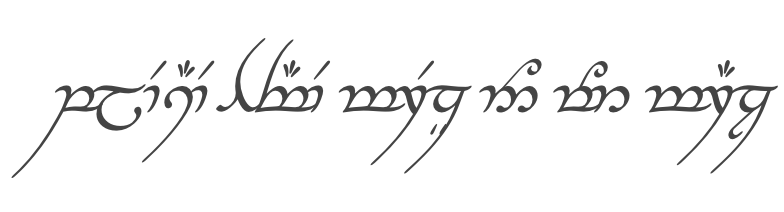
\includegraphics{ElvishPlea}\footnote{Originally I wanted to make all the variables Elvish too, but there were problems with the \LaTeX{} package and so I had to settle for including only the one sentence.}

\end{document}
